\section{Experiments}
\label{sec:experiments}

\subsection{Number of Iterations}
One of the major flaws in the graph net framework is the issue of determining how many iterations to run.
In theory, because of the universal approximation properties of neural nets, the optimal number of iterations is any number larger than the diameter of the graph, so that each node can make a fully informed decision knowing the entire graph topology.
However, this is not realistic: as shown in Figure~\ref{fig:dataset-graph-stats}, the maximum diameter of any of the graphs is above 200, meaning that we would have to run the graph neural net for an intractable number of iterations to be able to get the ``full'' result.
Instead, we approximate the result by running fewer iterations, theoretically losing out on certain classes of decisions (although further enforcing our inductive bias, since we believe that local nodes should be the primary ones that matter).
It is not immediately clear how we should choose the \textsc{\NIter} hyperparameter though.
We ran two experiments to try to select the ideal settings: a \emph{Bayesian Optimization} based approach, and what we call an \emph{Iteration Ensemble} approach.

\begin{figure}
  \centering
  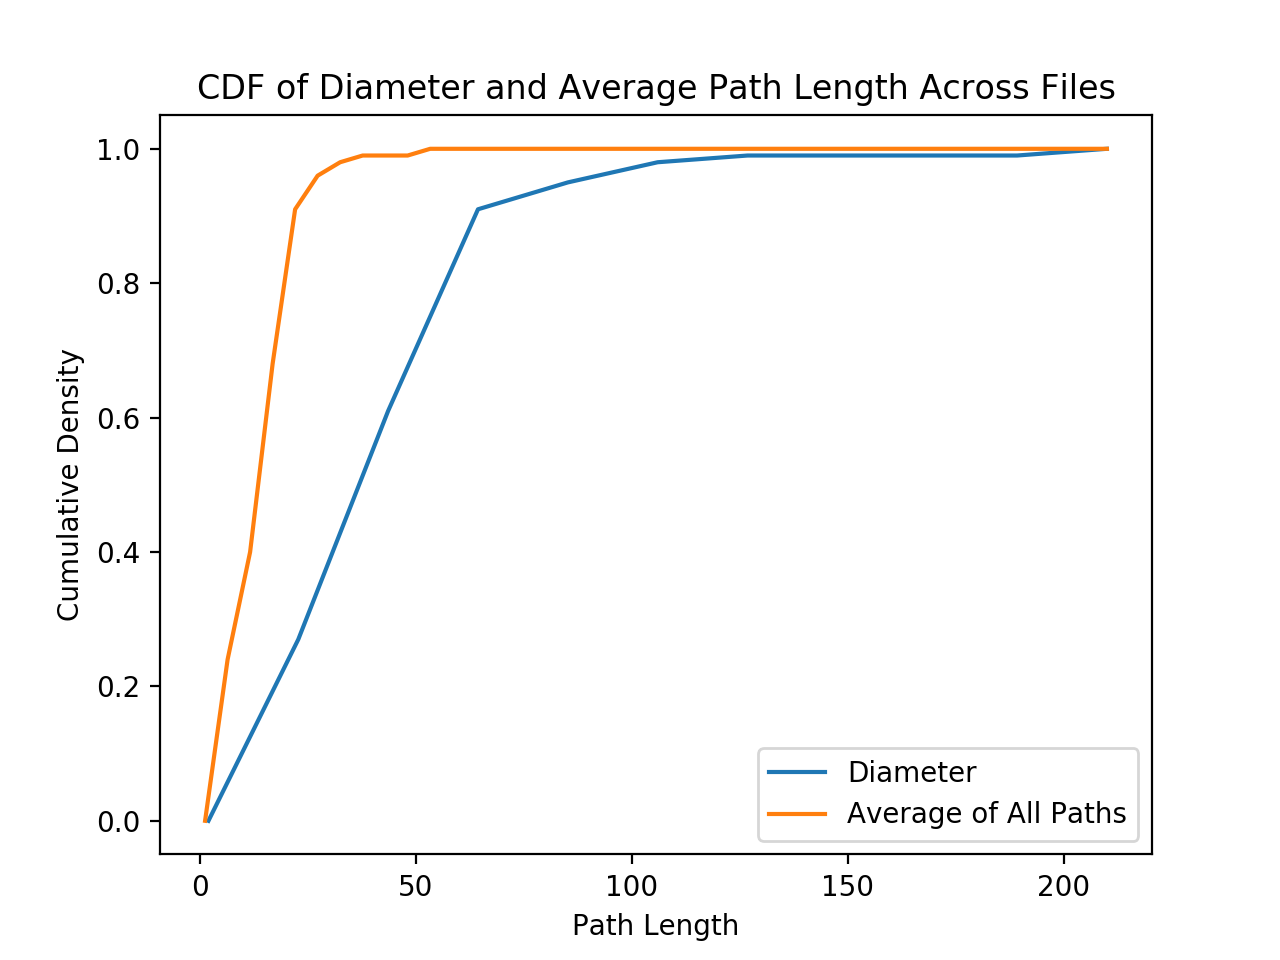
\includegraphics[width=0.49\linewidth]{img/diameter}
  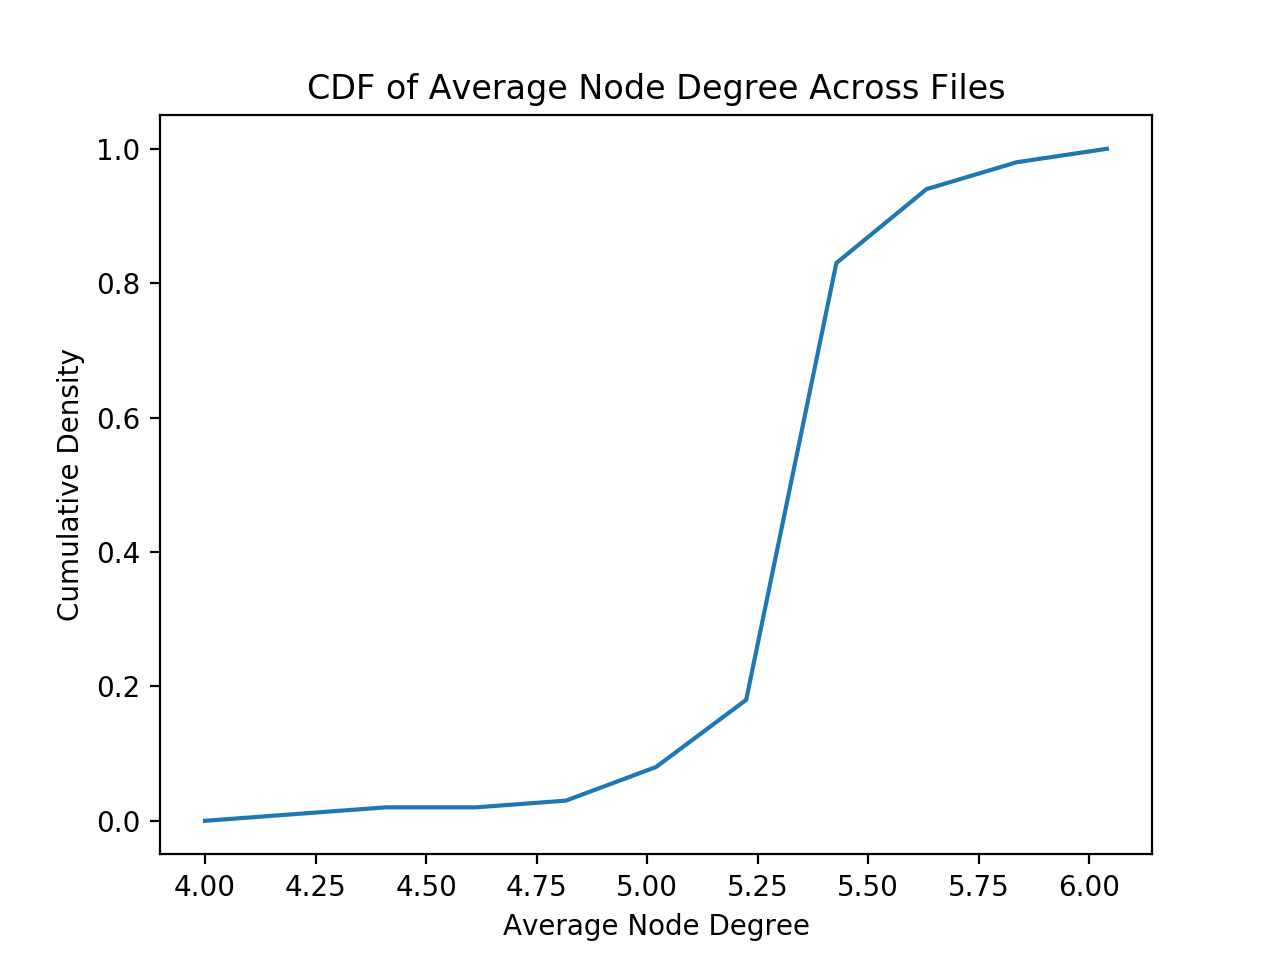
\includegraphics[width=0.49\linewidth]{img/node_degree}
  \caption{Generated graph statistics}
  \label{fig:dataset-graph-stats}
\end{figure}


Graph nets do not have the same guarantee as other approximation

\paragraph{Iteration Ensemble.}

\paragraph{Bayesian Optimization.}

\subsection{Edge Ablation}

\todo{Experiments, Results}

%%% Local Variables:
%%% TeX-master: "main"
%%% End: